\chapter{Background Research}
\label{chapter2}

\section{Robot Operating System (ROS)}

The Robot Operating System or ROS, is a flexible framework for writing robot software. It offers libraries aiming at simplifying common robotics tasks \cite{website:aboutROS}, which otherwise would be complex to achieve in such a broad field.

ROS is a collaborative and open-source project empowering the expertise of some of the best robotics institutions, laboratories and individuals around the globe \cite{website:aboutROS}, making ROS a well rounded framework for all types of robotics challenges. 

ROS comes in many versions. This project will make extensive use of the ROS Indigo Igloo version.

\section{TIAGo}

TIAGo, a robot by PAL Robotics, will be used to carry out the research project, which is rotating around navigation in human environments and human-robot interaction, making TIAGo a good fit.

In fact, TIAGo is a service robot designed to work in indoor environments \cite{website:TIAGo}, hence fitting our project aim of maneuvering and interacting around and with humans. 

Moreover, TIAGo's size and technical features make it an ideal platform for the research project, combining many of the necessary aspects for the positive outcome of the task, including mobility, perception and human-robot interaction capabilities \cite{website:TIAGo}.

\begin{figure}[!htbp]
\begin{center}
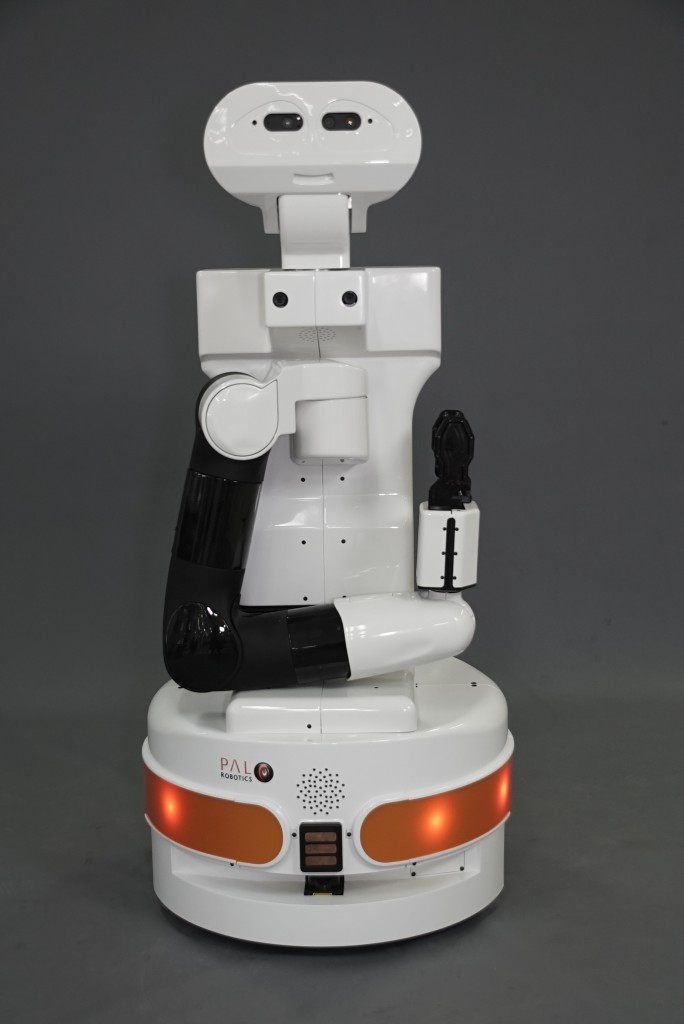
\includegraphics[width=3cm,height=4cm,keepaspectratio]{images/tiago.jpg}
\end{center}
\caption{TIAGo (Image taken from \cite{website:TIAGOWEBSITE}).}
\end{figure}

\section{Human Detection}

\subsection{Introduction}

After a first consideration for which model of choice should be used for the first phase of the project, consisting in TIAGo, the robot, being able to detect the presence of humans in the environment, in our case a room, a variety of different approaches have been tried so as to identify one with good accuracy and real-time performance.

The Histogram of Oriented Gradients (HoG) and its variances such as the Oriented Histograms of Flow and Appearance (OHFA) and the AdaBoosted versions were the first choices for the task, nonetheless the result obtained held a low accuracy in the detections with a lot of false positive and high latency during the real-time usage.

Hence, the choice to move towards a deep learning approach for the human detection task. At the time of the writing there are several state-of-the art neural network models for high detection accuracy for hundreds of different objects. The considered models include:

\begin{enumerate}
  \item YOLO \cite{paper:YOLO}
  \item Faster R-CNN \cite{paper:FRCNN}
  \item SSD \cite{paper:SSD}
\end{enumerate}

The difference in the level of accuracy between these networks is such that it doesn't play an important role in the decision of which model to choose for the task, instead the computational efficiency and speed of detection are what the task considers vital.

The SSD model is therefore chosen, given the available variations of the former for computationally restrained devices and its ease to be embedded in a system.

\subsection{SSD (Single Shot MultiBox Detector)}

The SSD is a single deep neural network able to detect various objects in a scene, by discretizing the output space with bounding boxes over different aspect ratios and scales \cite{paper:SSD}. In fact during the prediction process, a neural network feed-forward generates a score for the presence in the previously created boxes for each object category that the network has been trained on \cite{paper:SSD}. Further adjustments are carried out to better match the object.  

Overall, the SSD model approaches the detection task in a simpler way to other methods that require specific object proposals as for example Faster CNN \cite{paper:FRCNN}. Furthermore, because the process eliminates these RPN (Region Proposal Networks) and further pixel re-sampling, the model is able to fit the whole computation is a single network, making it easier to train and more integrable into vision applications \cite{paper:SSD}.

\subsection{SSD Model}

Current state-of-the-art object detection systems such as FRCNN \cite{paper:FRCNN} and YOLO \cite{paper:YOLO} are variances of the same detection process, which includes the following steps:

\begin{enumerate}
  \item Hypothesize bounding boxes
  \item Pixel or features re-sampling
  \item Classification
\end{enumerate}

Nonetheless this pipeline has proved to obtain great accuracy results when tested on the PASCAL, VOC and COCO datasets, it has as well confirmed its high computational cost when used in embedded systems, even with high-end hardware \cite{paper:SSD}, making it almost impossible to use in real-world applications which have limited resources.

The SSD model solves partially the computational problem by improving upon the pipeline without loosing any accuracy. The enhancement comes from the transformation of the region proposal layer into a small convolutional filter which is able to predict object categories and bounding boxes' offsets within the same network. Moreover, separate filters are used to carry the same detection process but at different aspect ratios making the detection of smaller or partially occluded objects possible. Below the SSD model architecture is presented, before describing the different parts to it:

\begin{figure}[!htbp]
\begin{center}
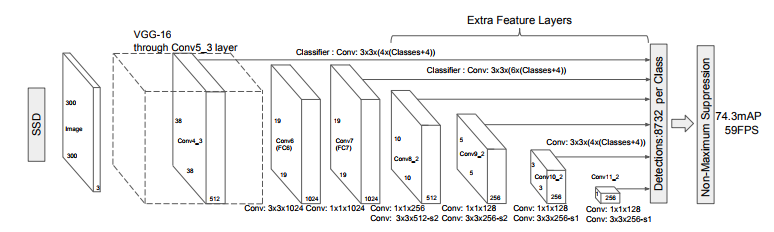
\includegraphics[width=\linewidth]{images/ssd_architecture.png}
\end{center}
\caption{SSD Model (Image taken from: \cite{paper:SSD})}
\label{fig:sshModel}
\end{figure}

The general SSD approach is based on a feed-forward convolutional network that at first creates a fixed-size collections of bounding boxes and scores for the presence of object instances in those boxes, followed by a non-maximum suppression step to produce the final detections \cite{paper:SSD}.

This general approach can be broken up  into small steps, each carried by a specific layer in the network. The early network layers, called \textbf{base network} which in the SSD case is a \textbf{VGG-16}, are used for image classification tasks \cite{paper:SSD}. An auxiliary structure is then added to the base network to produce detections with the following key features for the detections \cite{paper:SSD}:

\begin{enumerate}
  \item Multi-scale feature maps
  \item Convolutional predictors
  \item Default boxes and aspect ratios
\end{enumerate}

\textbf{Multi-scale feature maps}

Convolutional feature layers are added at the end of the VGG-16 truncated network with the aim of decreasing the input image size progressively allowing for detections at multiple scales \cite{paper:SSD}

\textbf{Convolutional predictors}

Every added feature layer (discussed previously) can produce a fixed set of detection predictions \cite{paper:SSD}. Generally a feature layer of size m x n with p channels requires a 3 x 3 x p kernel to produce either a score for a category or a bounding box offset relative to the image \textbf{Ground Truth} box.

\textbf{Default boxes and aspect ratios}

A set of default bounding boxes is set for each feature map cell. For each feature map cell the offsets relative to the default box shapes as well as the per-class scores indicating the presence of a class instance in each of those boxes \cite{paper:SSD}. Specifically, for each box out of k, the \textit{c} class score is computed as well as the 4 offsets (for each discretised point of the original image 4 bounding boxes are draw with different aspect ratios), yielding (\textit{c} + 4)kmn outputs for a m x n feature maps \cite{paper:SSD}.

\begin{figure}[!htbp]
\begin{center}
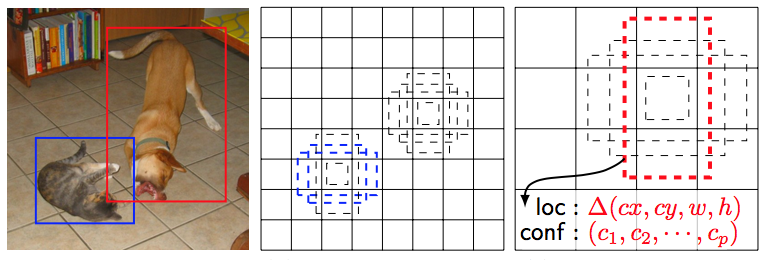
\includegraphics[width=\linewidth]{images/gt_boxes.png}
\end{center}
\caption{Ground truth, feature maps, offset computation(Image taken from: \cite{paper:SSD}).}
\label{fig:ssdGT}
\end{figure}

\section{MobileNets}

Deep convolutional neural network have been made a standard in nowadays computer vision techniques, thanks to the power of data and the fast computations available. In fact, after the 2012 AlexNet challenge, when these neural networks where first popularized, the general trend has become to make these deeper and more complicated \cite{paper:MobileNets} to improve the overall accuracy.

Nonetheless, the following advances are not taking into consideration the limitations that these more accurate and complicated structure have in real world applications such as this research project, where object recognition tasks need to be carried in real-time on a computationally limited platform \cite{paper:MobileNets}.

MobileNet provides an efficient network architecture in order to build small and low latency models that can be easily embedded in vision applications running on limited devices \cite{paper:MobileNets}.

\subsection{MobileNet Architecture}

The MobileNet structure is built on top of a depthwise separable convolutions except for the first layer which is full convolutional layer \cite{paper:MobileNets}. Such a simplistic approach permits the further discovery of possible network topologies for a better performance overall. The MobileNet architecture is preseted below:

\begin{figure}[!htbp]
\begin{center}
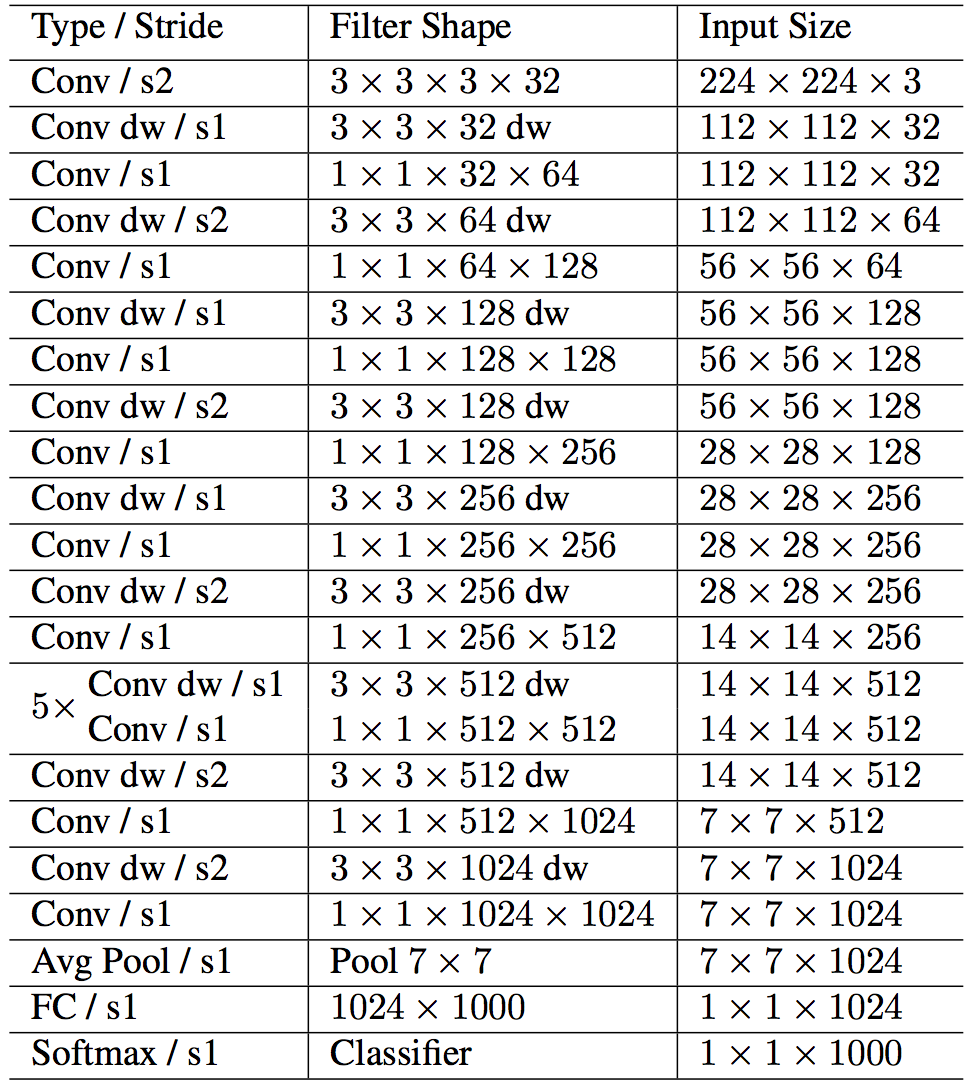
\includegraphics[width=7cm,height=9cm,keepaspectratio]{images/mobileNet_structure.png}
\end{center}
\caption{MobileNet Architecture (Image taken from: \cite{paper:MobileNets}).}
\end{figure}

Each component in the in the network is followed by a batch-normalisation and a rectified linear unit with the sole exception of the final layer which feeds directly into the softmax layer for classification\cite{paper:MobileNets}. Furthermore, the down sampling is handled with strided convolutions in the depthwise convolutions as well as in the first layer \cite{paper:MobileNets}, while a final average pooling does reduce the overall spatial resolution to 1 before the fully connected layer \cite{paper:MobileNets}. In total the MobileNet counts 28 layers.

\begin{figure}[!htbp]
\begin{center}
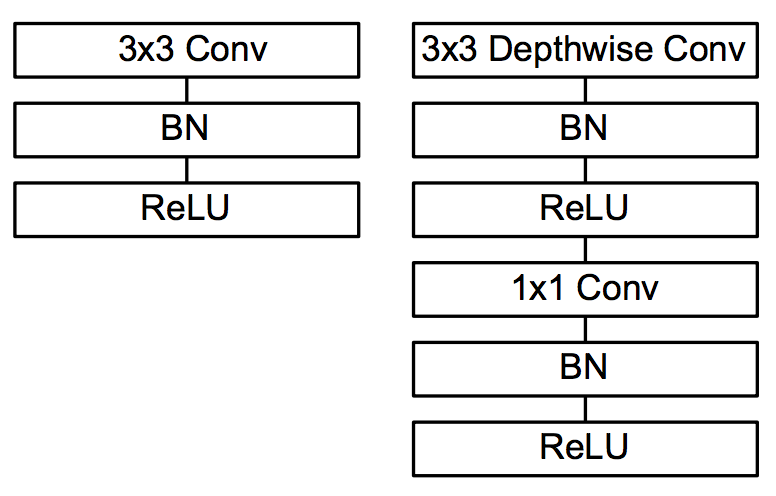
\includegraphics[width=7cm,height=9cm,keepaspectratio]{images/mobileNet_contrast.png}
\end{center}
\caption{Standard convolutional (left), Depthwise Separable convolutions (right) (Image taken from: \cite{paper:MobileNets}).}
\end{figure}

\subsection{Depthwise Separable Convolution}

The depthwise separable convolutions is a factorized convolutions which factorize a standard convolution into a depthwise convolution and a 1x1 convolution called pointwise convolution \cite{paper:MobileNets}.

The main difference between a usual convolution and the depthwise one is that the former applies both a filtering and combination procedure to the set of inputs into a new set of outputs in a single step \cite{paper:MobileNets} while the latter splits the procedure into two separate layers. This separation drastically reduces the computation and model size. The figure below shows a standard convolution (a), a depthwise convolution (b) and a 1x1 pointwise convolution (c).

\begin{figure}[!htbp]
\begin{center}
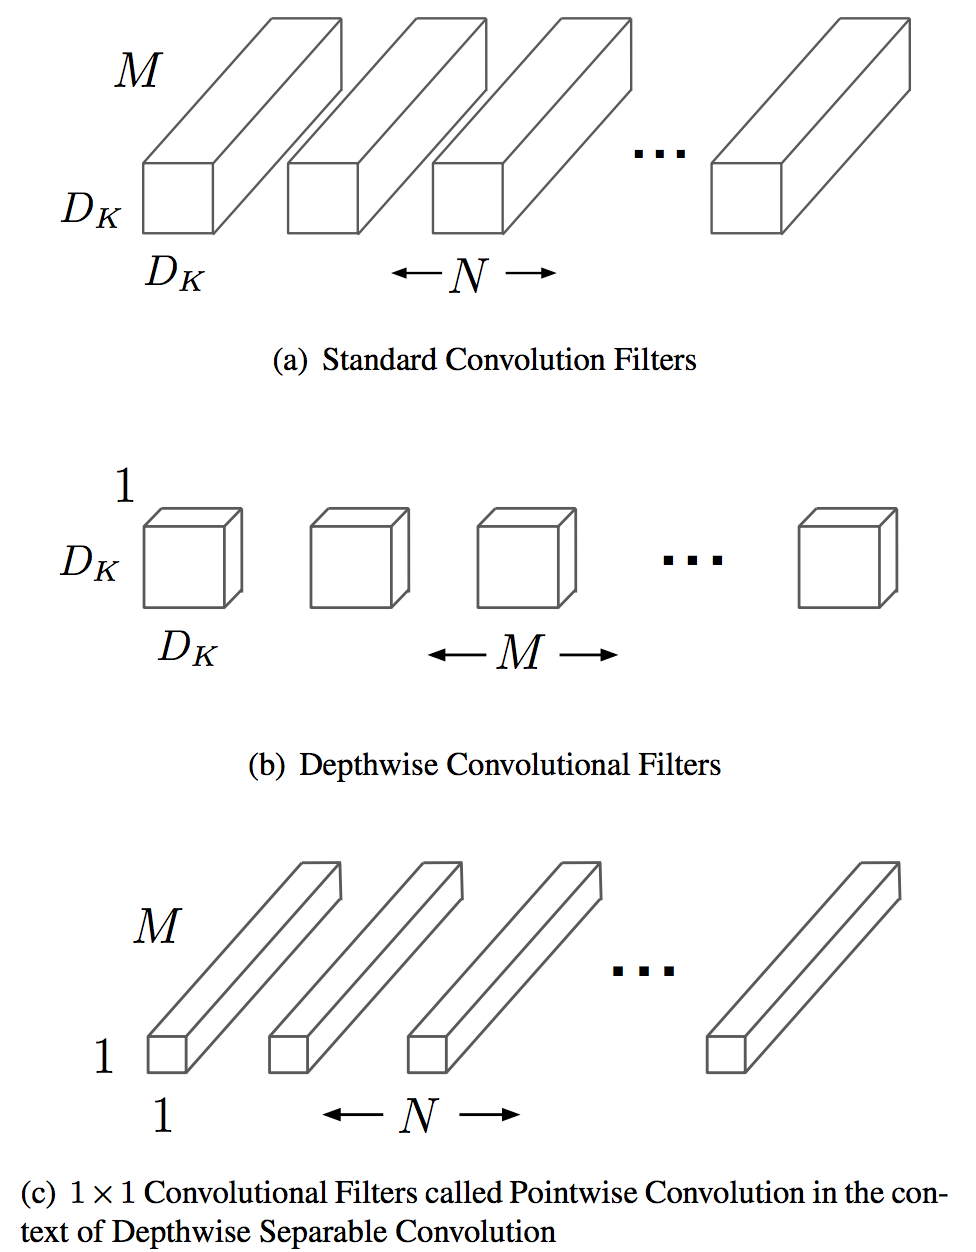
\includegraphics[width=5cm,height=7cm,keepaspectratio]{images/convolutions.png}
\end{center}
\caption{Convolution transformation (Image taken from: \cite{paper:MobileNets}).}
\end{figure}

\subsection{Width and Resolution Multipliers}

The basic mobileNet architecture already offers a better efficiency by being smaller and with a lower latency than the usual networks. Nonetheless, many times specif applications require a model which is even smaller and less computationally expensive. The width and resolution hyper-parameters serve exactly this.

The  width multiplier defined with the greek letter \textit{alpha} has the role to thin the network layers uniformly \cite{paper:MobileNets}. Usual values for \textit{alpha} are between 0 and 1, with 1 being the model baseline for mobileNet. Moreover, the smaller the parameter gets, the smaller the model will be and hence the less accurate, therefore a trade off has to be found.

The second hyper-parameter to reduce the computational cost of a general neural network is the resolution multiplier defined with the greek letter p \cite{paper:MobileNets}. The parameter is directly applied to the input image and the internal representation of every layer is subsequently reduced by the same multiplier \cite{paper:MobileNets}. Typical values for p are between 0 and 1, with 1 being the mobileNet baseline.

Both parameters reduce the computational cost quadratically.

\begin{figure}[!htbp]
\begin{center}
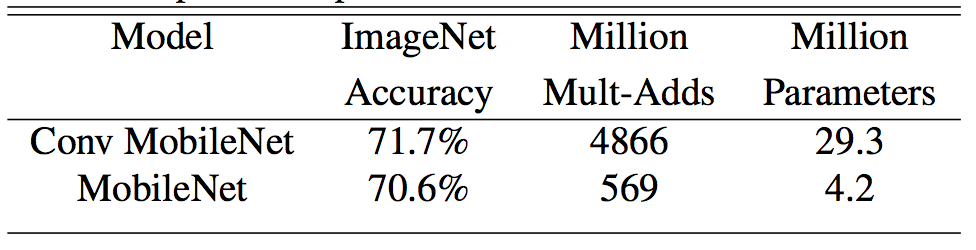
\includegraphics[width=10cm,height=10cm,keepaspectratio]{images/mobileNet_table.png}
\end{center}
\caption{Full vs Depthwise convolutions performance (Image taken from: \cite{paper:MobileNets}).}
\end{figure}

\section{Human-Robot Navigation}

One major design goal in human-robot interaction is the ability of the robot to behave in an intelligent manner \cite{paper:JOINDISCUSSION}. The majority of the navigation systems focus quite exclusively on the task of reaching a certain position, however, when considering intelligent agents which coexist with humans these two challenges can't be treated separately \cite{paper:JOINDISCUSSION}.

The mission to be accomplished consists in the robot being able to enter a room, approach a group of people engaged in a discussion and maintain a behavioral discussion, where this means executing similar moving patterns to the persons involved in the discussion.

\subsection{Psychological Considerations}

Such autonomous systems, which are going to coexist with humans are deeply influenced by human psychology, for the simple reason that these systems will have to behave like us \cite{paper:JOINDISCUSSION}. Human interactions in particular are bounded to specific rules depending of the type of conversation and on the level of confidentiality that the people have within the conversation itself, which mainly defines the distance between the individuals. Moreover, particular shapes are adopted by people when these are involved in a discussion. The system will hence have to take into considerations all these criteria \cite{paper:JOINDISCUSSION}.

\subsection{Topological Map and State Diagram}

The navigation system will make use of a topological map to initiate navigational actions \cite{paper:JOINDISCUSSION}. The map is represented as a graph structure containing edges and nodes, respectively representing map locations and behavioral tasks such as \textit{approach} and \textit{join}. An example of such a topological map is show below:

\begin{figure}[!htbp]
\begin{center}
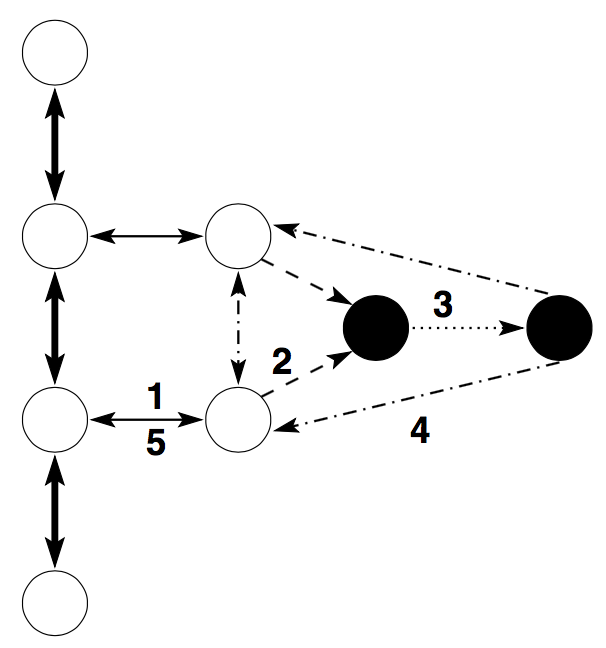
\includegraphics[width=6cm,height=8cm,keepaspectratio]{images/topological.png}
\end{center}
\caption{Representation of the states and space during navigation (Image taken from: \cite{paper:JOINDISCUSSION}).}
\end{figure}

\subsection{Control}

Once the topological map has been defined for desired environment, which given the simplicity of the representation requires a limited amount of time to construct a new one \cite{paper:JOINDISCUSSION}, the second part to the system consists in making the robot perform the following actions:

\begin{enumerate}
  \item Approach the group of people
  \item Maintain a discussion formation
\end{enumerate}

After the robot has entered the room in question a human detection module is initiated. This module along with multiple view geometry helps the estimation of the position in the map of the individual, from which the direction and distance can be derived.

As soon as the robot has reached the group of people, the individual persons must be detected in order to keep a certain formation \cite{paper:JOINDISCUSSION}. Sonar reading are used to accomplish the task. In fact, nearby persons are reconstructed from the echos in ascending order based on their distance from the robot \cite{paper:JOINDISCUSSION}. Orientations of the individuals in the robot frame are then recovered and used to adapt the robot position depending on the vicinity of the persons.